%%
%% Appendix Skript AfuTUB-Kurs von Sebastian Lange <dl7bst@dk0tu.de>
%%      Lizenz CC BY-NC-SA (Attribution-NonCommercial-ShareAlike 4.0)
%%      https://creativecommons.org/licenses/by-nc-sa/4.0/legalcode
%%
%% 02.11.2017 DL7BST V.01
%%
%% Anhang
%%
%%%%%%%%%%%%%%%%%%%%%%%%%%%%%%%%%%%%%%%%%%%%%%%%%%%%%%%%%%%%%%%%%%%%%

\chapter{Formelsammlung Klasse A}
    \label{att:formela}

    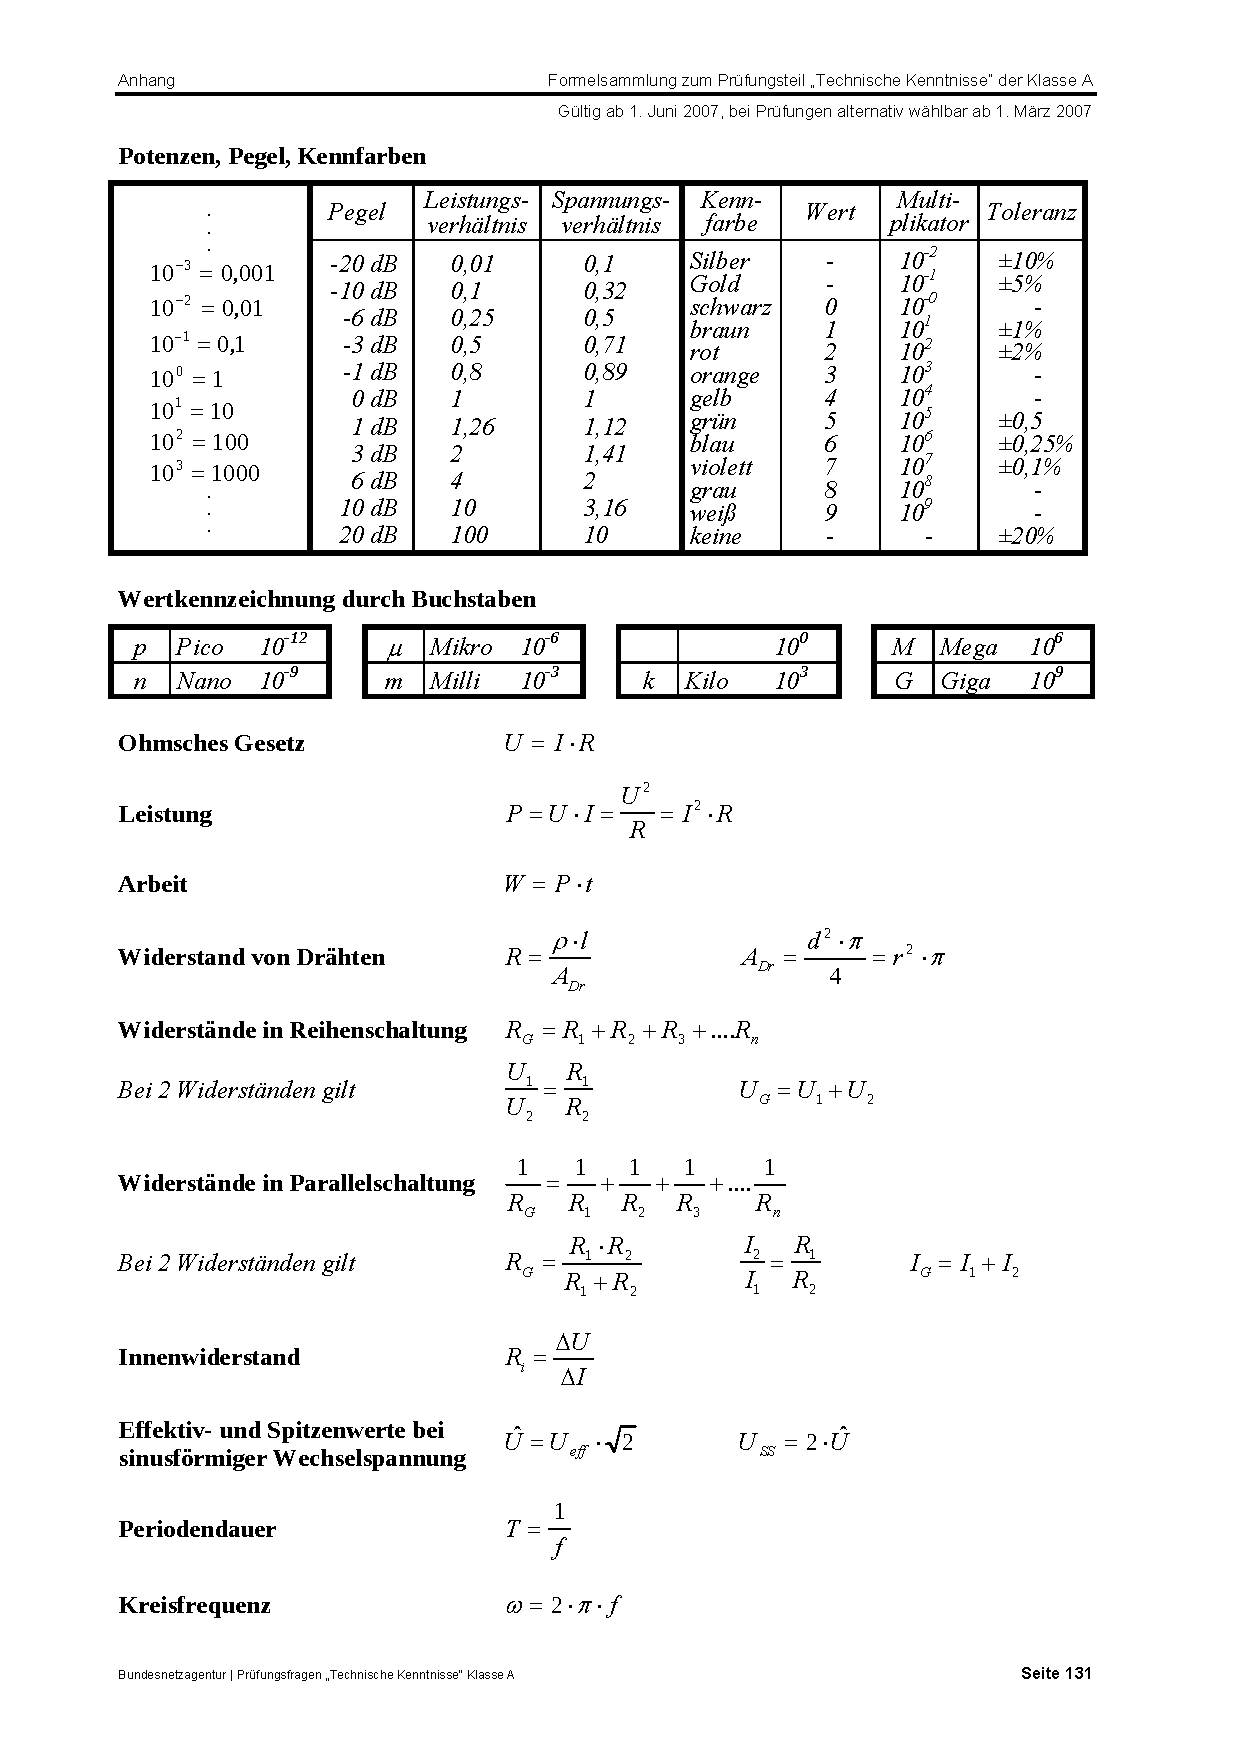
\includepdf[pages=-]{appendix/formulary/Formelsammlung_A_2007.pdf}

% TODO Besser als einzelne Bilder einbinden?
%    \begin{figure}[h]
%        \centering
%        \includegraphics[width=0.63\textwidth]{Rapporteur}
%        \caption{Azimutwinkelmaß \cite{rapporteur1}}
%        \label{fig:rapporteur1}
%    \end{figure}
%
%    \begin{figure}[h]
%        \centering
%        \includegraphics[width=0.63\textwidth]{Rapporteur_180deg}
%        \caption{Elevationswinkelmaß \cite{rapporteur2}}
%        \label{fig:rapporteur2}
%    \end{figure}

\clearpage\newpage ~

%%%%%%%%%%%%%%%%%%%%%%%%%%%%%%%%%%%%%%%%%%%%%%%%%%%%%%%%%%%%%%%%%%%%%

\chapter{Formelsammlung Klasse E}
    \label{att:formele}

    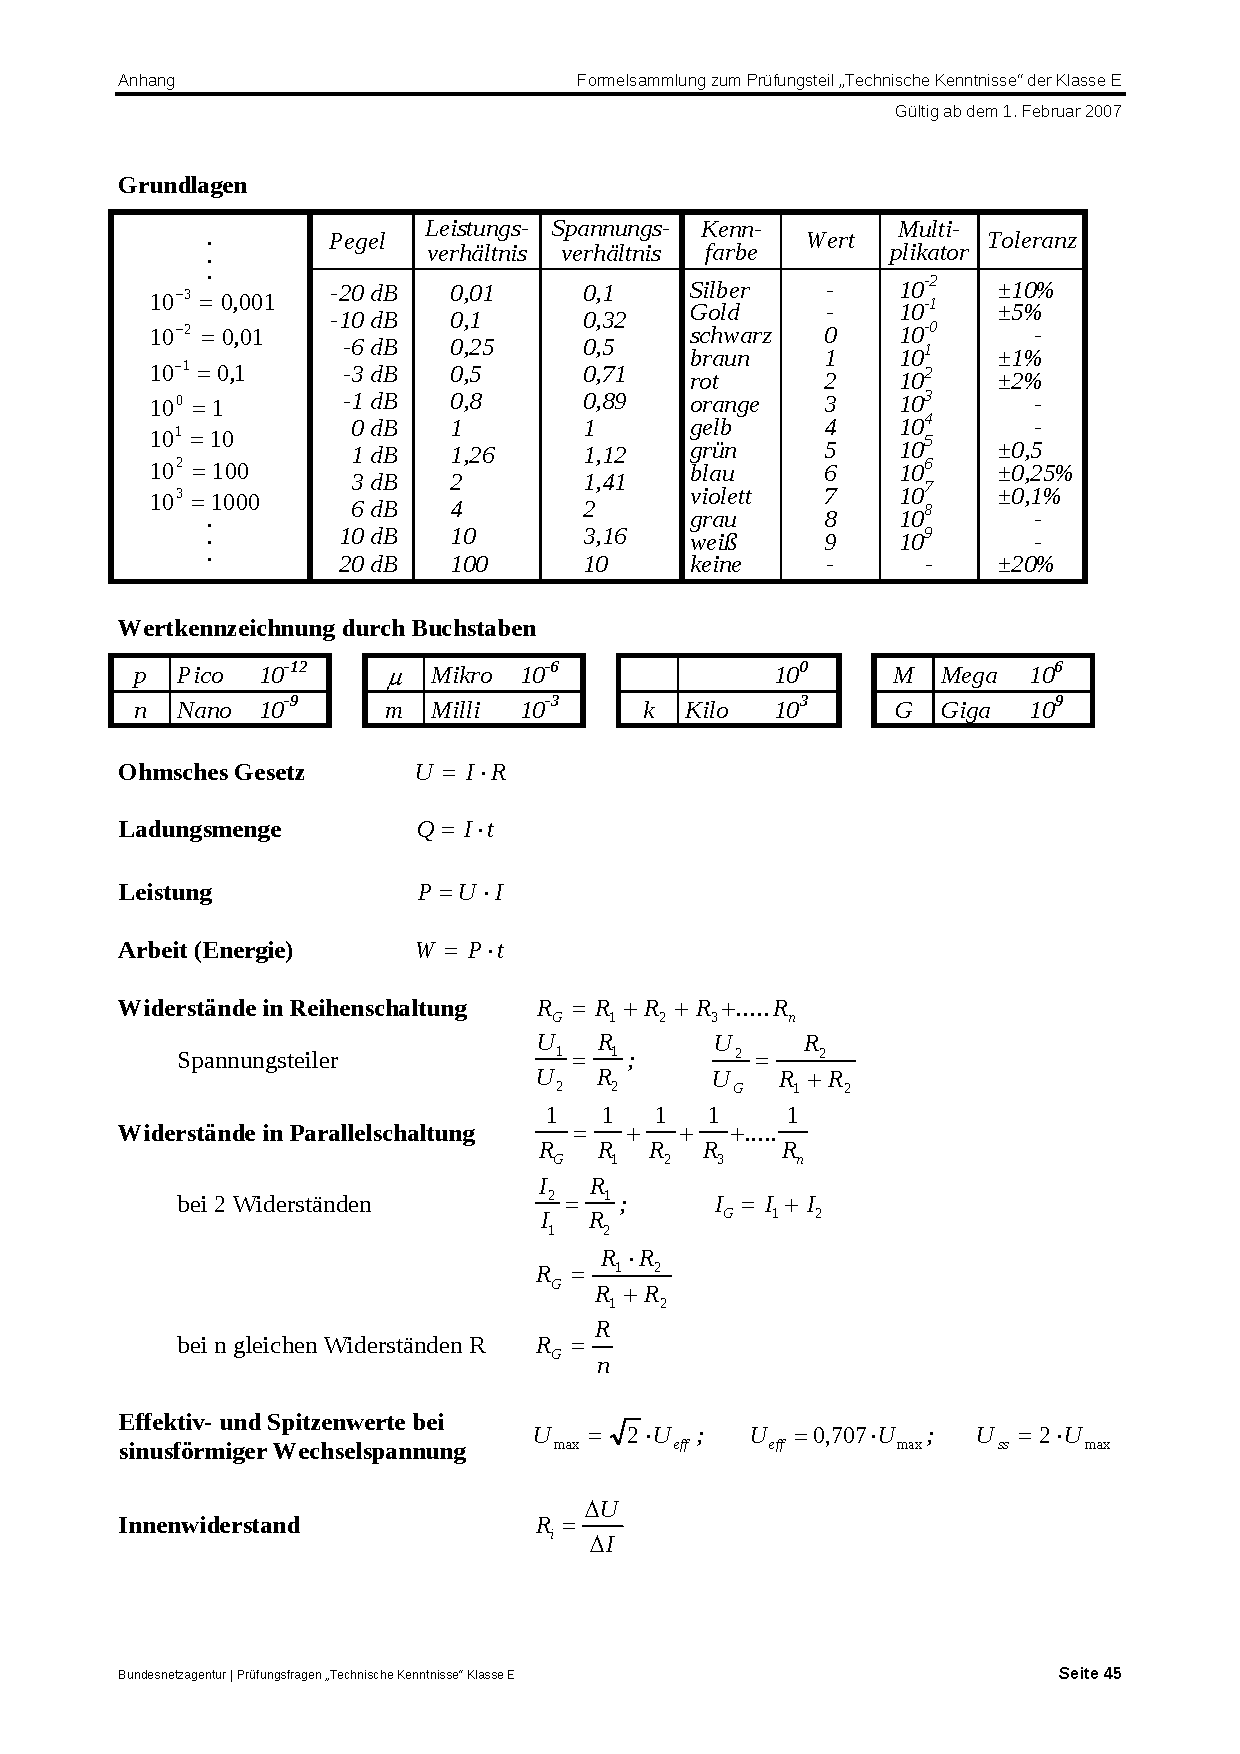
\includepdf[pages=-]{appendix/formulary/Formelsammlung_E_2007.pdf}

\clearpage\newpage ~

%%%%%%%%%%%%%%%%%%%%%%%%%%%%%%%%%%%%%%%%%%%%%%%%%%%%%%%%%%%%%%%%%%%%%

\chapter{Formelsammlung Zusatz}
    \label{att:formel+}

    \section*{Potenzen, Pegel, Kennfarben}

    Die Formelsammlung der BNetzA lässt sich nur für Widerstände im
    4-Ringe-Farbsystem heranziehen. Deshalb ergänzend für die Praxis mit 5 oder
    6 Ringen ist Tabelle \ref{fig:r-farbcode} heranzuziehen.

    \begin{figure}[h]
        \centering
        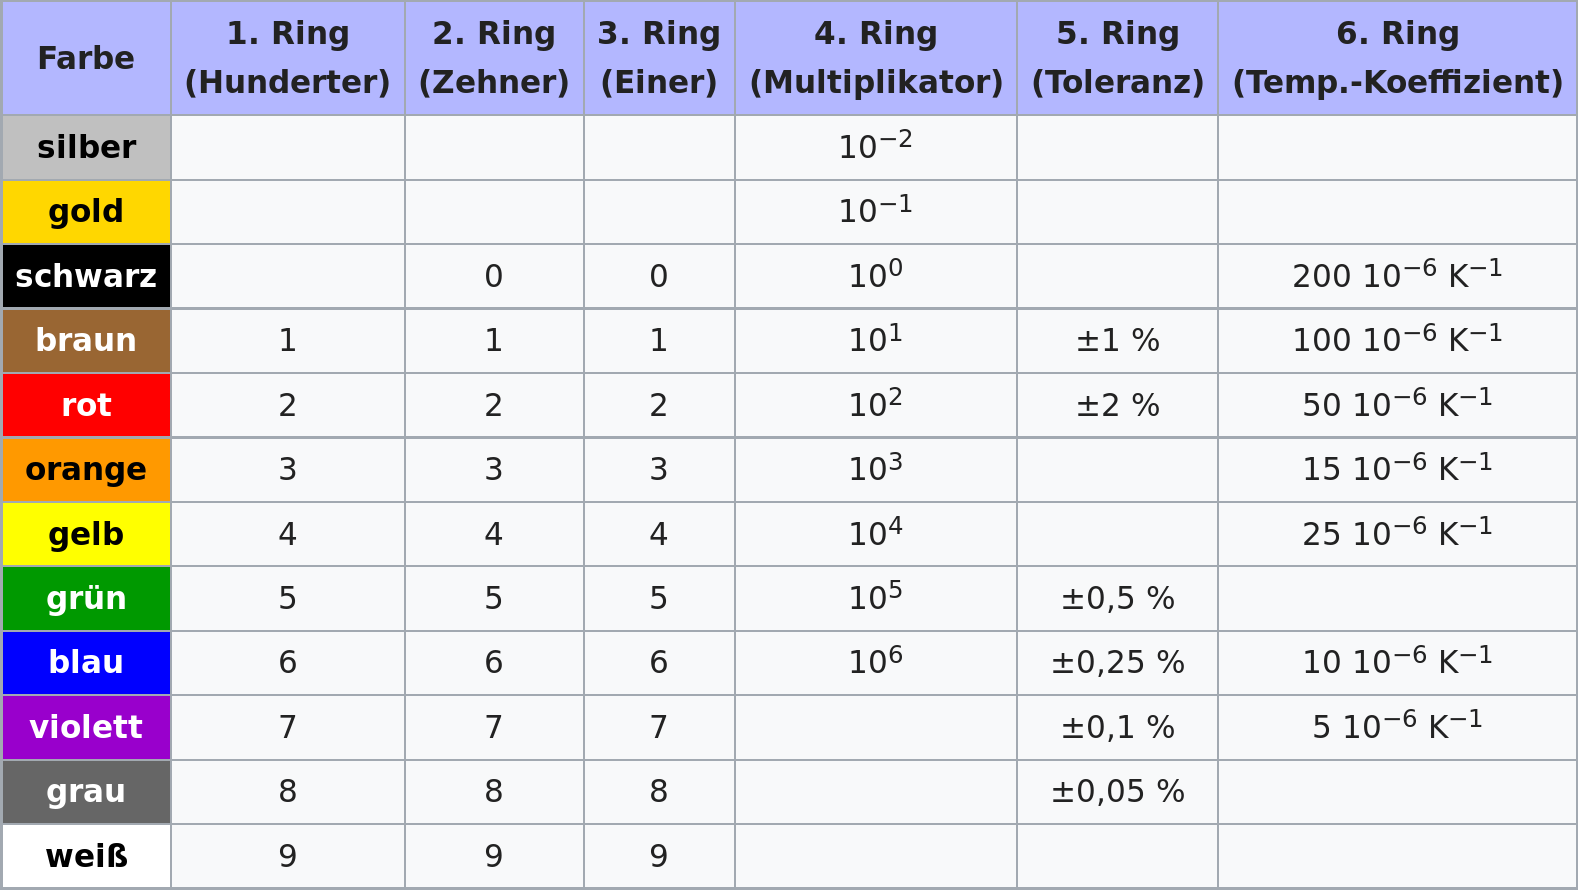
\includegraphics[width=0.8\textwidth]{appendix/formulary/R-Farbcode.png}
        \caption{Farbkodierung von Widerständen mit 5 oder 6 Ringen \cite{wpwiderstand}}
        \label{fig:r-farbcode}
    \end{figure}

\clearpage\newpage ~

%%%%%%%%%%%%%%%%%%%%%%%%%%%%%%%%%%%%%%%%%%%%%%%%%%%%%%%%%%%%%%%%%%%%%

\chapter{Datasheet: Drehkondensator ModulBus VCap4}
    \label{att:vcap}

    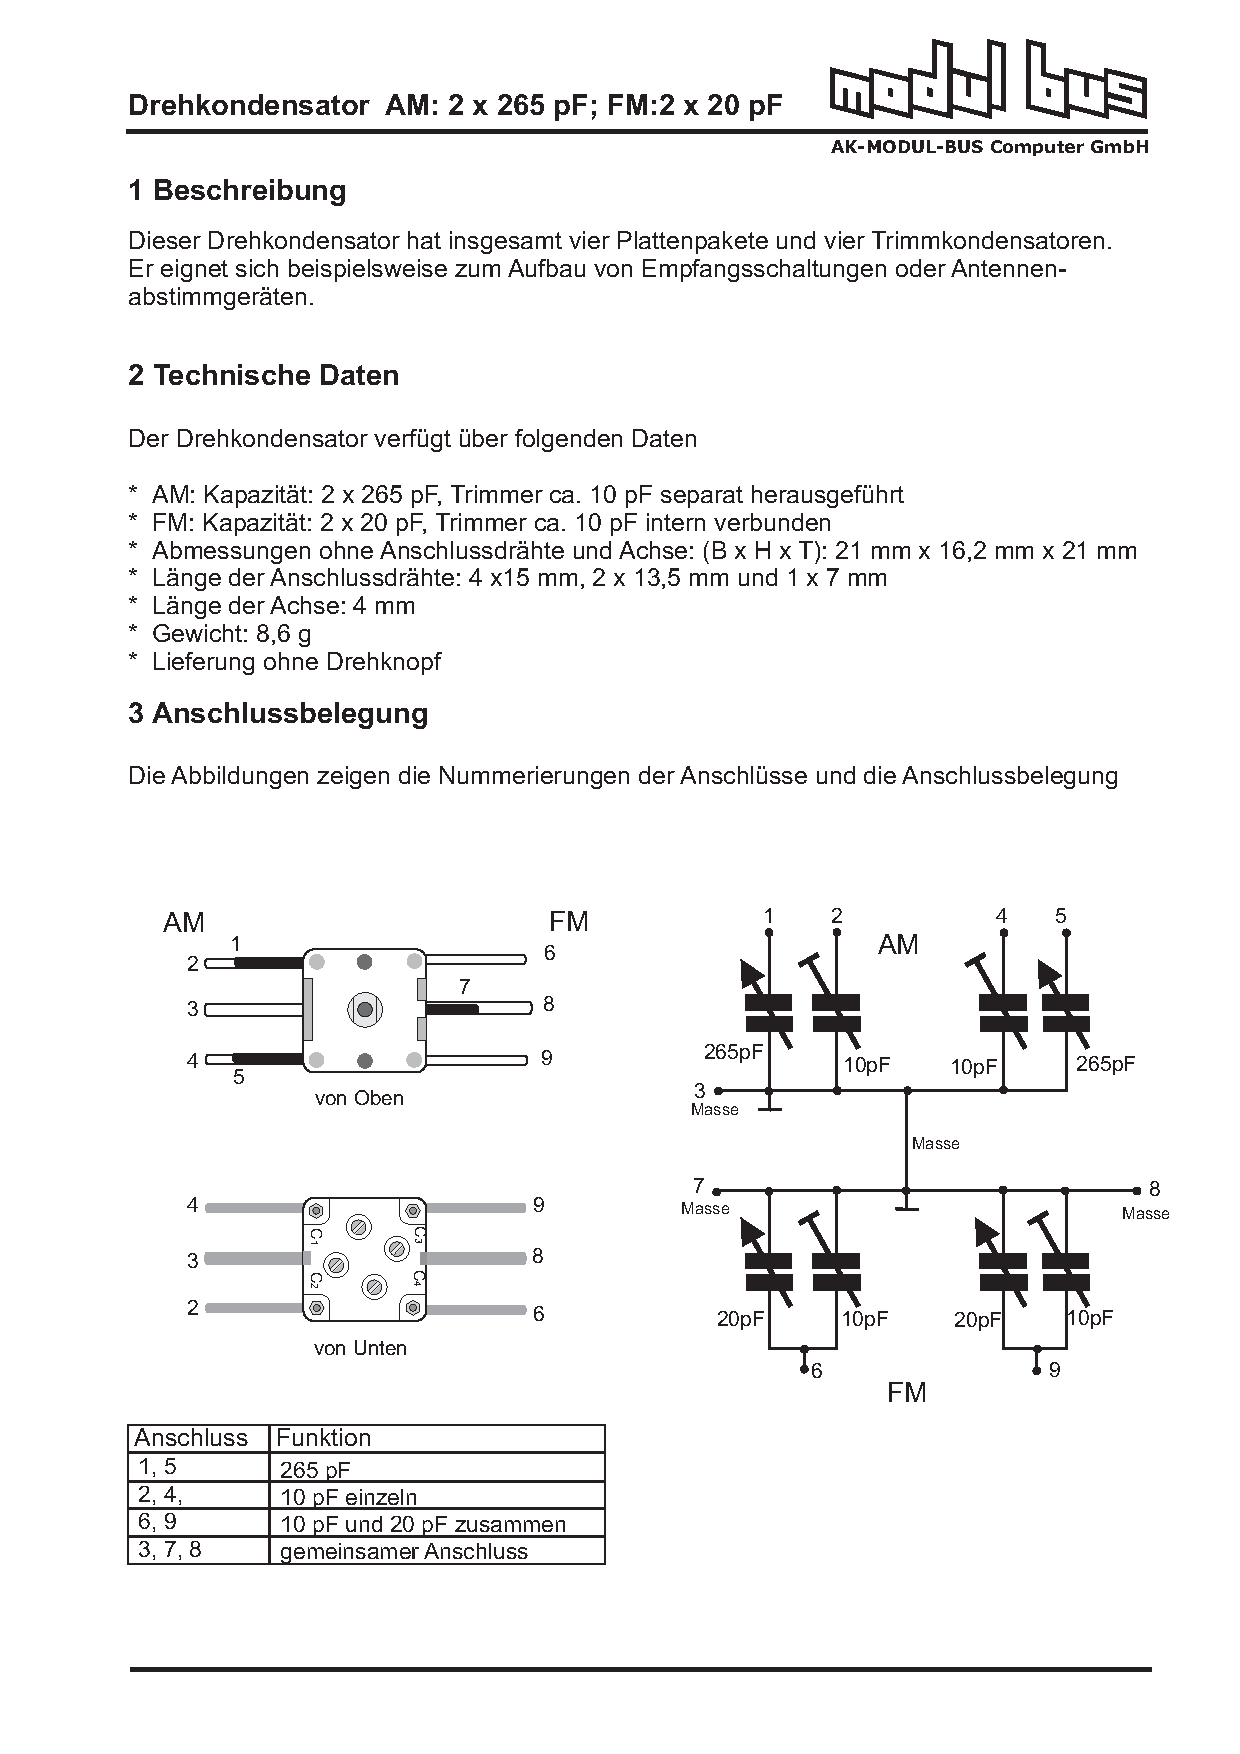
\includepdf[pages=-]{appendix/datasheets/vcap4_ModulBus.pdf}

\clearpage\newpage ~

%%%%%%%%%%%%%%%%%%%%%%%%%%%%%%%%%%%%%%%%%%%%%%%%%%%%%%%%%%%%%%%%%%%%%

\chapter{Manual LC-Meter Ascel Æ20204}
    \label{att:ae20204}

    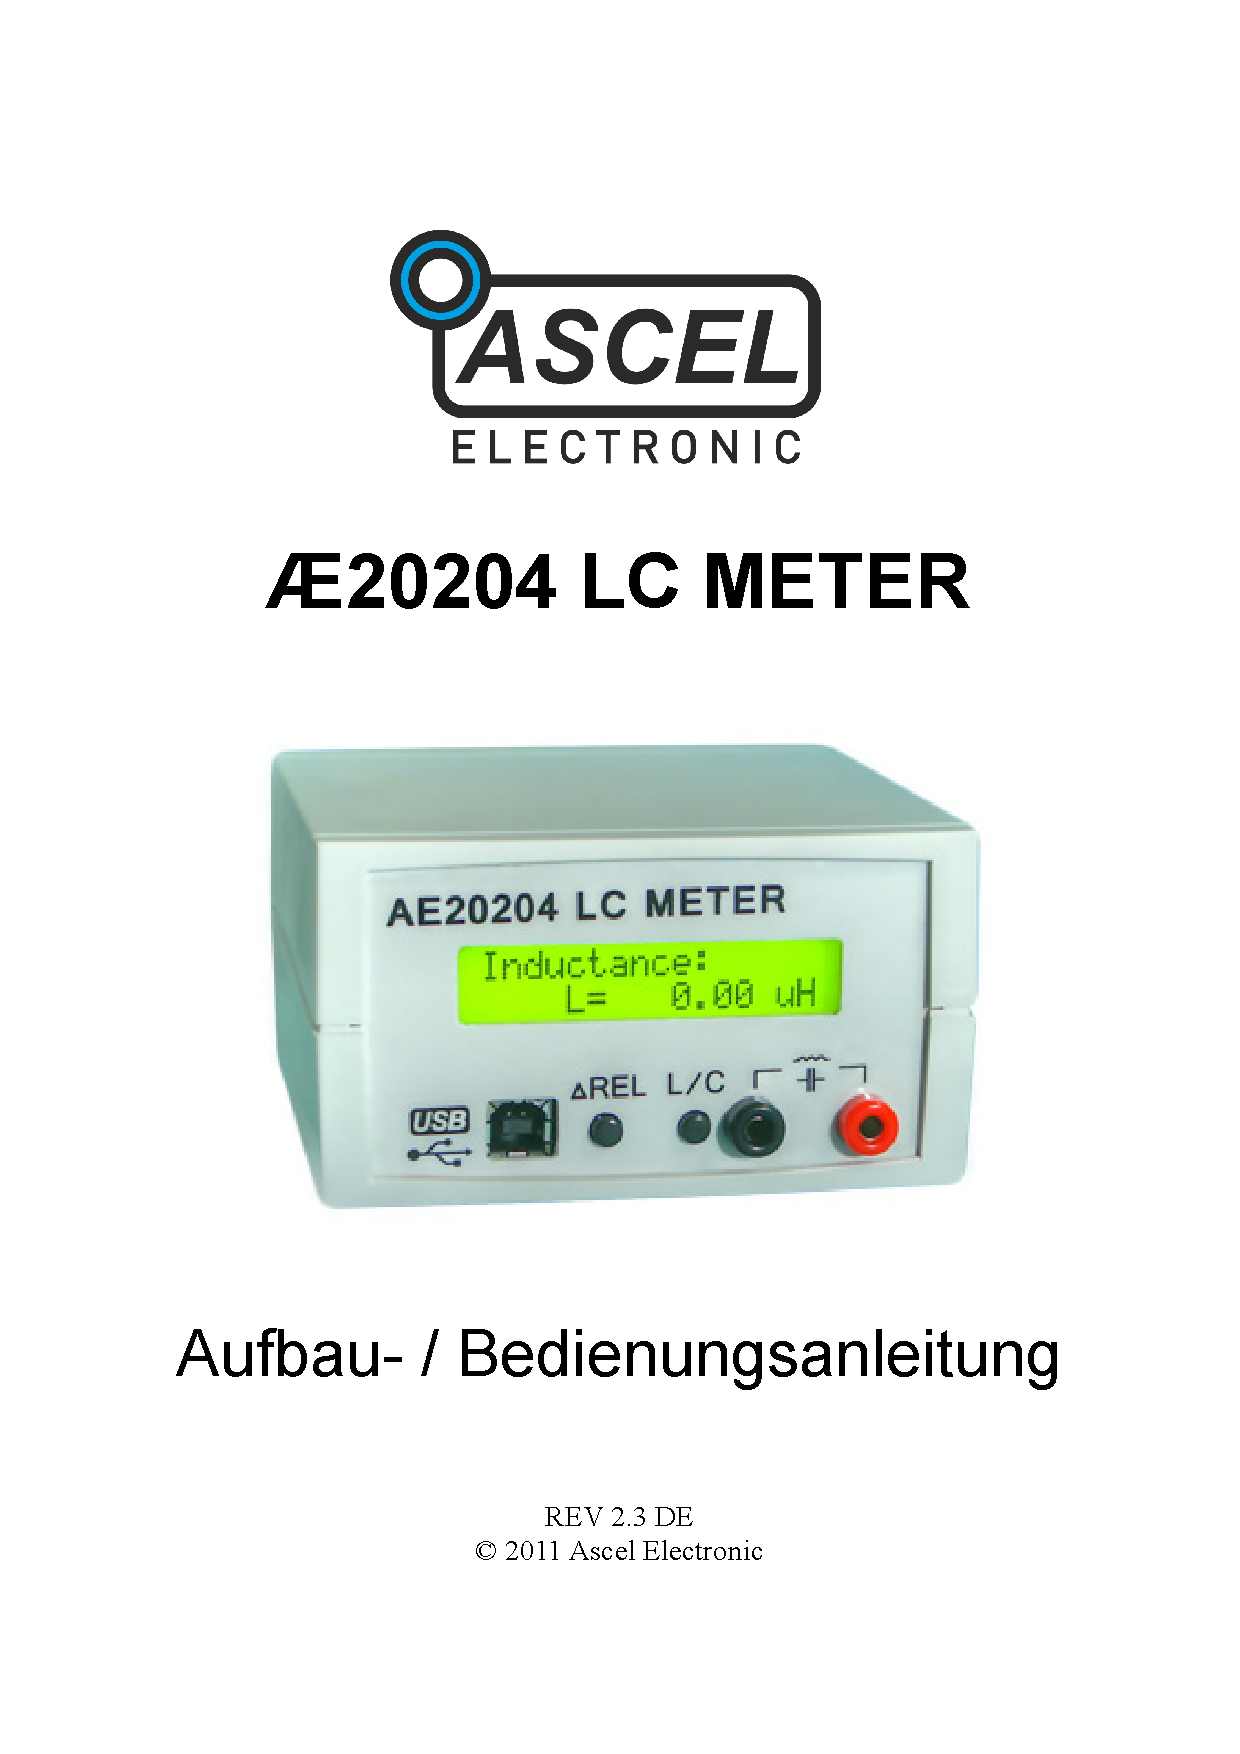
\includepdf[pages=-]{appendix/manuals/ae20204_manual_de_1+8+9+32-34.pdf}

\clearpage\newpage ~
